\section{NuWro}

\begin{slide}[toc=NuWro MC]{NuWro MC event generator}
\null\vfill  
  
  \vspace{-10pt}
  \begin{center}
    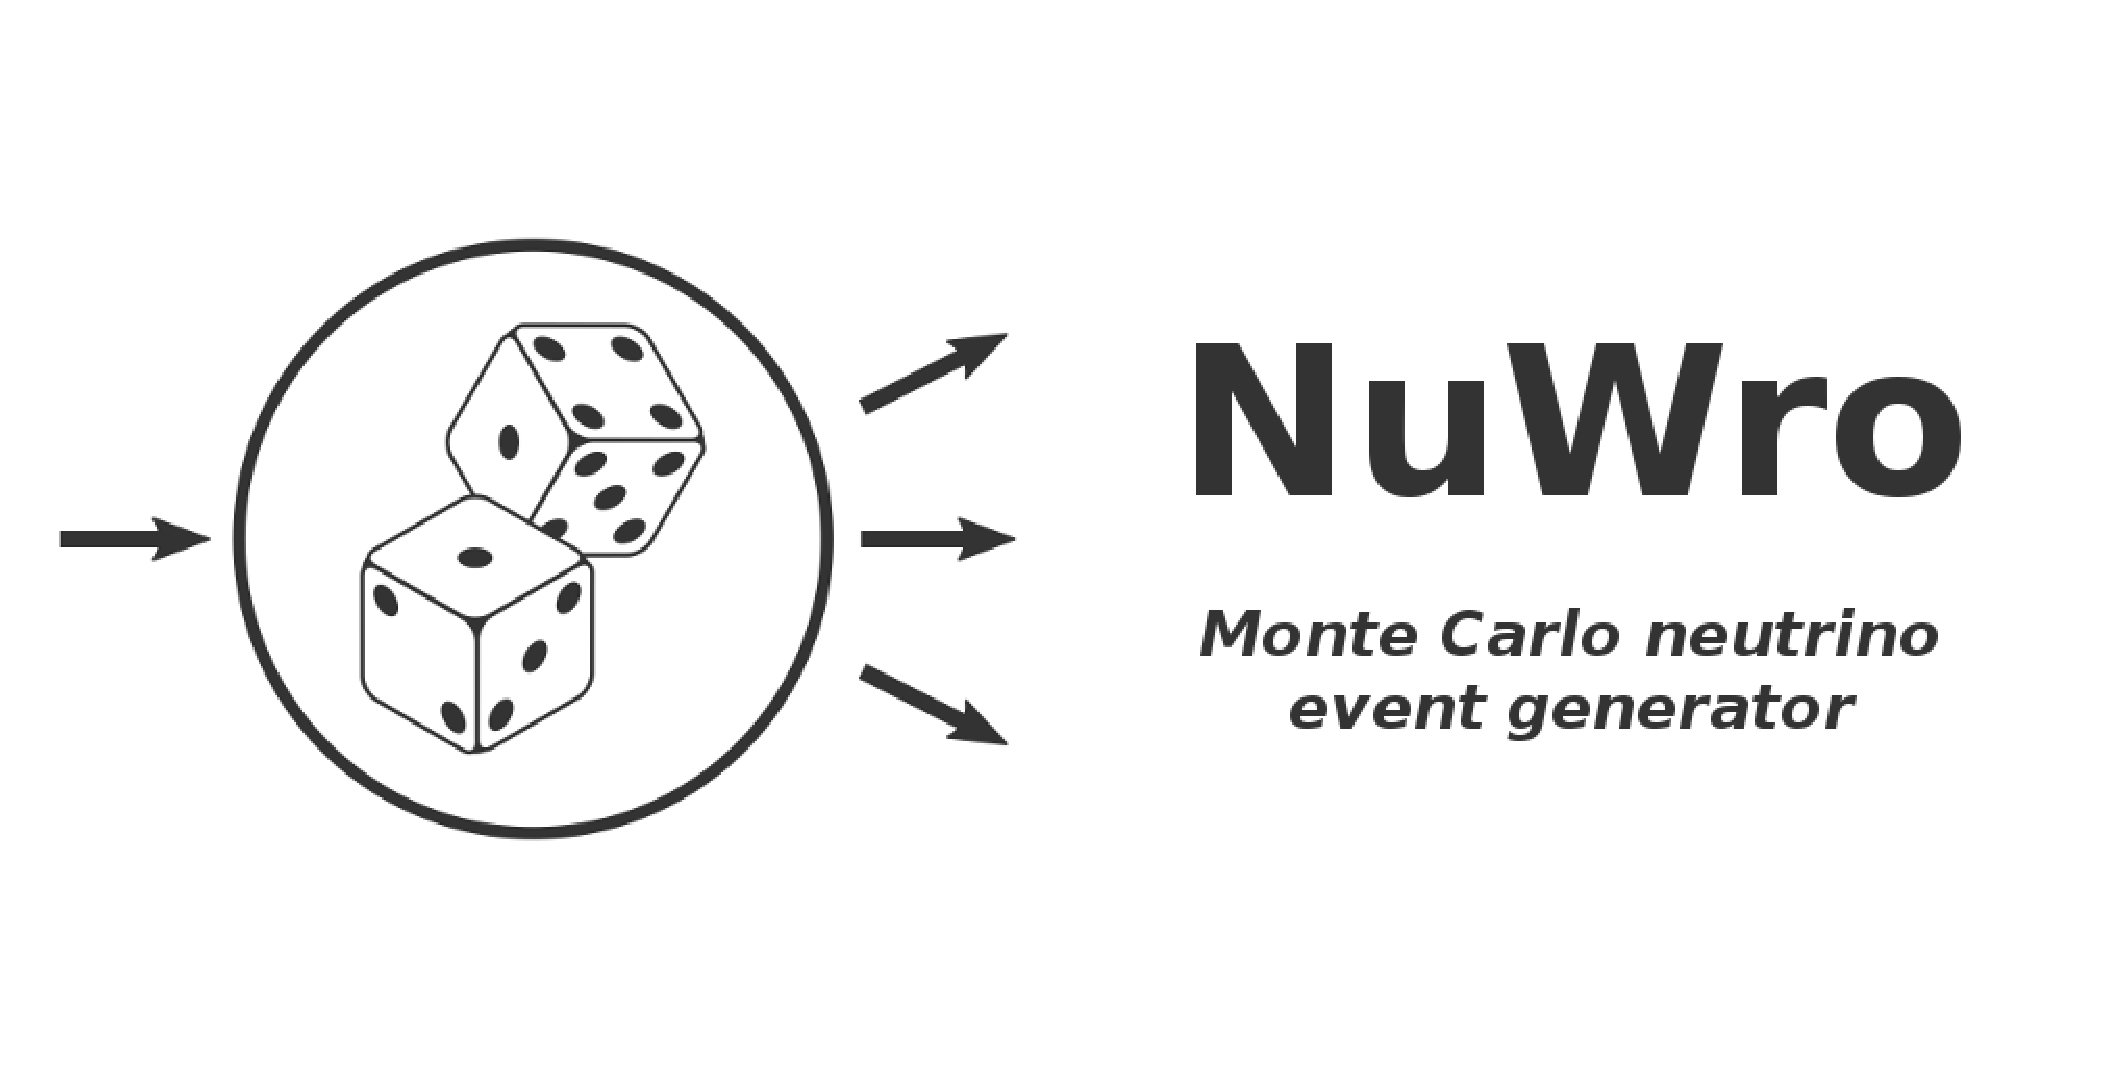
\includegraphics[width=0.75\columnwidth]{img/nuwro.eps}
  \end{center}
  \vspace{-30pt}
  {\it\hfill\grey{formerly known as WroNG}}
  
  \sep
  
  \begin{itemize}

    \item It has been developed at Wroclaw University since 2006
    \item The authors were encouraged by prof. Danuta Kie{\l}czewska from Warsaw University
    \item It is written in {\it\small C++} and uses {\it\small ROOT} library to store the output
    \item The open source code can be downloaded from the repository: \url{https://github.com/nuwro/}
%    \item (Local) Fermi Gas, as well as Spectral Function, can be used for the description of nucleons momenta.
%    \item Intranuclear cascade is available for nucleons and pions.
%    \item final state interactions are implemented.
%    \item Realistic beam models (eg T2K) and ability to use detector geometry read from a {\it\small ROOT} file (tested with T2K ND280 and MINERvA).
    
  \end{itemize}

\vfill\null
\end{slide}

%%%%% NuWro package %%%%%

\begin{emptyslide}[toc=]{}
\null\vfill

\centering\usetikzlibrary{mindmap,trees}

\tikzstyle{fullAngle}[1] = [level #1/.append style = {sibling angle = 360/\the\tikznumberofchildren}]
\tikzstyle{angle60}[1] = [level #1/.append style = {sibling angle = 60}]

\tikzset{level 1 concept/.append style = {font = \large, sibling angle = 90, level distance = 5cm, minimum size = 2.5cm}}
\tikzset{level 2 concept/.append style = {font = \normalsize, sibling angle = 60, level distance = 3.5cm, minimum size = 2cm}}
\tikzset{level 3 concept/.append style = {font = \small, sibling angle = 60, level distance = 3cm, minimum size = 2cm}}
\tikzset{level 4 concept/.append style = {font = \small, sibling angle = 60, level distance = 3cm, minimum size = 2cm}}

\scalebox{0.5}
{
\begin{tikzpicture}

  \path[mindmap, concept color = pdcolor1, text = pdcolor2]
  
  node[concept, minimum size = 1cm] {\Large\bf NuWro} [clockwise from = 90]
  child[concept color = pdcolor3!100!pdcolor1]
  {
    node[concept] {Interactions} [clockwise from = -150]
    child { node[concept] {QEL} }
    child { node[concept] {``RES''} }
    child { node[concept] {``DIS''} }
    child { node[concept] {MEC} }
    child { node[concept] {COH} }
  }  
  child[concept color = pdcolor5!100!pdcolor1]
  {
    node[concept] {Other} [clockwise from = 30]
    child {node[concept] {eWro} }
    child {node[concept] {NuWro on-line} }
  }
  child[concept color = pdcolor4!100!pdcolor1]
  {
    node[concept] {Nuclear Effects} [clockwise from = -30, level 2 concept/.append style = {sibling angle = 120}]
    child[concept]
    {
      node[concept] {Nucleus Model} [clockwise from = 30]
      child { node[concept] {Fermi Gas} }
      child { node[concept] {Spectral Function} }
    }
    child[concept]
    {
      node[concept] {FSI} [clockwise from = -150]
      child {node[concept] {Pions} }
      child { node[concept] {Nucleons} }
    }
  }
  child[concept color = pdcolor6!100!pdcolor1]
  { 
    node[concept] {Experiment} [clockwise from = -150]
    child {node[concept] {Beam} }
    child { node[concept] {Detector} }
  };

\end{tikzpicture}
}

\vfill\null
\end{emptyslide}

%%%% DYNAMICS %%%%%

\begin{wideslide}[toc=Dynamics]{Implemented dynamics}

  \rput(9.5,-3){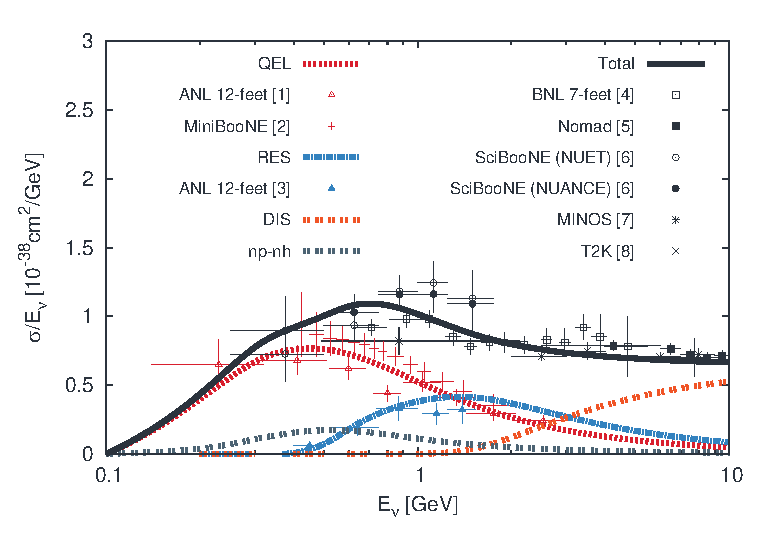
\includegraphics[width = 0.6\columnwidth]{img/xsec_cc2.eps}}

    
    \begin{itemize}
     \item All major interaction channels \\ are implemented, for charged and \\ neutral current, covering \\ neutrino energy region from \\ a few hundreds MeV \\ (Impulse Approximation limit) \\ to several TeV:
    \end{itemize}

%      \vspace{10pt}

      \begin{itemize}
	\addtolength{\itemindent}{10pt}
      
	\item[QEL] \red{(quasi-)elastic scattering}
	
	\item[RES] \blue{pion production through \\ \hspace{10pt}a $\Delta$ resonance excitation}
	
	\item[DIS] \orange{more inelastic processes}
	
	\item[COH] coherent pion production

	\item[np-nh] \grey{two body current contribution} %\\ \hspace{10pt}(Transverse Enhancement use on the plot).
      
      \end{itemize}

    \vspace{65pt}
    \rput[l](6.5,4.5){\color{pdcolor3}\footnotesize [1] PRD 19 (1979) 2521}
    \rput[l](6.5,4){\color{pdcolor3}\footnotesize [2] PRD 81 (2010) 092005}
    \rput[l](6.5,3.5){\color{pdcolor3}\footnotesize [3] PRD 16 (1977) 3103}
    \rput[l](6.5,3){\color{pdcolor3}\footnotesize [4] PRD 25 (1982) 617}
    \rput[l](10,4.5){\color{pdcolor3}\footnotesize [5] PLB 660 (2008) 19}
    \rput[l](10,4){\color{pdcolor3}\footnotesize [6] PRD 83 (2011) 012005}
    \rput[l](10,3.5){\color{pdcolor3}\footnotesize [7] PRD 81 (2011) 072002}
    \rput[l](10,3){\color{pdcolor3}\footnotesize [8] PRD 87 (2013) 092003}

\end{wideslide}

%%%%% QEL %%%%%%

\begin{slide}[toc=(Q)EL scattering]{(Quasi-)elastic scattering}
\null\vfill
  
  \twocolumn
  {
    \begin{itemize}
     \item Llewellyn-Smith model is used for charged current quasi-elastic scattering
     \item Not much difference here between generators (but default parameters)
    \end{itemize}
  }
  {
    \scalebox{0.75}{\begin{tikzpicture}[node distance = 1cm and 1.5cm]
  
 \node(left) [] {};
 \node(leftEmpty) [left=of left] {};
 \node(leftUp) [above=of leftEmpty] {$\nu / l$};
 \node(leftDown) [below=of leftEmpty] {$\nu$};
 
 \node(right) [right=of left] {};
 \node(rightEmpty) [right=of right] {};
 \node(rightUp) [above=of rightEmpty] {N'};
 \node(rightDown) [below=of rightEmpty] {N};
 
 \draw[curl, thick] (left.center) -- node[above] {$Z^0 / W^\pm$} ++ (right.center);
 
 \draw[color = pdcolor1, thick] (left.center) -- (leftUp);
 \draw[color = pdcolor1, thick] (left.center) -- (leftDown); 
 \draw[color = pdcolor1, thick] (right.center) -- (rightUp);
 \draw[color = pdcolor1, thick] (right.center) -- (rightDown);
 
\end{tikzpicture}
}
  }
  
  \sep
  
  \twocolumn
  {
    \centering\scalebox{0.5}{\begin{tikzpicture}
  
  \node (n) [circle, filled, minimum width = 4cm] {};

  \node (q1) [circle, filled={pdcolor5}, minimum width = 1cm, below=of n, yshift = 4.75cm] {}; 
  \node (q2) [circle, filled={pdcolor6}, minimum width = 1cm, below=of q1, xshift = 1cm] {}; 
  \node (q3) [circle, filled={pdcolor7}, minimum width = 1cm, below=of q1, xshift = -1cm] {};
 
  \draw [curl={pdcolor2}, very thick] (q1) -- (q2);
  \draw [curl={pdcolor2}, very thick] (q2) -- (q3);
  \draw [curl={pdcolor2}, very thick] (q3) -- (q1);

\end{tikzpicture}
}
  }
  {
    \sep
    \begin{itemize}
     \item Nucleon structure is parametrized by form factors
    \end{itemize}
  }

  \begin{itemize}
    \item Vector $\rightarrow$ Conserved Vector Current (CVC)
    \item Pseudo-scalar $\rightarrow$ Partially Conserved Axial Current (PCAC)
    \item Axial $\rightarrow$ dipole form with one free parameter (axial mass, $M_A$)
  \end{itemize}

  
\vfill\null
\end{slide}

%%%%% RES %%%%%

\begin{slide}[toc=RES pion production]{Resonance pion production}
\null\vfill

  \twocolumn
  {
    \begin{itemize}
      \item Most of generators (like NEUT and GENIE) uses Rein-Sehgal model
      \item RS model describes single pion production through baryon resonances below $W = 2$~GeV
    \end{itemize}
  }
  {
    \centering\scalebox{0.75}{\begin{tikzpicture}[node distance = 1cm and 1.5cm]
  
 \node(left) [] {};
 \node(leftEmpty) [left=of left] {};
 \node(leftUp) [above=of leftEmpty] {$\nu / l$};
 \node(leftDown) [below=of leftEmpty] {$\nu$};
 
 \node(right) [right=of left] {};
 \node(rightEmpty) [right=of right] {};
 \node(rightDown) [below=of rightEmpty] {N};

 \node(delta) [above=of rightEmpty, xshift = -1.0cm, yshift = -0.5cm] {$\Delta$};
 \node(rightUp1) [above=of delta, yshift = -0.5cm] {$\pi$};
 \node(rightUp2) [right=of delta, xshift = -1.0cm] {N'};
 
 \draw[curl, thick] (left.center) -- node[above] {$Z^0 / W^\pm$} ++ (right.center);
 
 \draw[color = pdcolor1, thick] (left.center) -- (leftUp);
 \draw[color = pdcolor1, thick] (left.center) -- (leftDown); 
 \draw[color = pdcolor1, thick] (right.center) -- (rightDown);
 \draw[color = pdcolor1, thick] (right.center) -- (delta);
 \draw[color = pdcolor1, thick] (delta) -- (rightUp1);
 \draw[color = pdcolor1, thick] (delta) -- (rightUp2);
 
\end{tikzpicture}
}
  }	

  \begin{itemize}
    \item In NuWro Adler-Rarita-Schwinger formalism is used to calculate $\Delta$ resonance explicitly
    \item Non-resonant background is estimated using quark-parton model
  \end{itemize}

\vfill\null
\end{slide}

%%%%% DIS %%%%%%

\begin{slide}[toc=Deep Inelastic Scattering]{Deep inelastic scattering [DIS]}
\null\vfill

  \twocolumn
  {
    \sep
    \begin{itemize}
     \item Quark-parton model is used for deep inelastic scattering
     \item Bodek-Young modification to the parton distributions at low $Q^2$ is included by most generators
    \end{itemize}
  }
  {
    \scalebox{0.75}{\begin{tikzpicture}[node distance = 1cm and 1.5cm]
  
 \node(left) [] {};
 \node(leftEmpty) [left=of left] {};
 \node(leftUp) [above=of leftEmpty] {$\nu / l$};
 \node(leftDown) [below=of leftEmpty] {$\nu$};
 
 \node(right) [right=of left] {};
 \node(rightEmpty) [right=of right] {};
 \node(rightDown) [below=of rightEmpty, xshift = -0.2cm, yshift = 0.2cm] {\scalebox{0.2}{\begin{tikzpicture}
  
  \node (n) [circle, filled, minimum width = 4cm] {};

  \node (q1) [circle, filled={pdcolor5}, minimum width = 1cm, below=of n, yshift = 4.75cm] {}; 
  \node (q2) [circle, filled={pdcolor6}, minimum width = 1cm, below=of q1, xshift = 1cm] {}; 
  \node (q3) [circle, filled={pdcolor7}, minimum width = 1cm, below=of q1, xshift = -1cm] {};
 
  \draw [curl={pdcolor2}, very thick] (q1) -- (q2);
  \draw [curl={pdcolor2}, very thick] (q2) -- (q3);
  \draw [curl={pdcolor2}, very thick] (q3) -- (q1);

\end{tikzpicture}
}};

 \node(rightUp) [above=of rightEmpty, xshift = -0.2cm, yshift = 0.2cm] {\scalebox{0.2}{\begin{tikzpicture}
  
  \node (center) {};
  
  \node [circle, filled={pdcolor4}, minimum width = 1cm, below=of center, xshift = 3cm, yshift = 0cm] {}; 
  \node [circle, filled={pdcolor5}, minimum width = 1cm, below=of center, xshift = 6cm, yshift = 1cm] {}; 
  \node [circle, filled={pdcolor6}, minimum width = 1cm, below=of center, xshift = 2cm, yshift = 2cm] {}; 
  \node [circle, filled={pdcolor7}, minimum width = 1cm, below=of center, xshift = 0cm, yshift = 3cm] {}; 
  \node [circle, filled={pdcolor4}, minimum width = 1cm, below=of center, xshift = 1cm, yshift = 4cm] {}; 
  \node [circle, filled={pdcolor5}, minimum width = 1cm, below=of center, xshift = 4cm, yshift = 3.5cm] {}; 
  \node [circle, filled={pdcolor6}, minimum width = 1cm, below=of center, xshift = 2.5cm, yshift = 3.5cm] {}; 
  \node [circle, filled={pdcolor7}, minimum width = 1cm, below=of center, xshift = 4.25cm, yshift = 1.5cm] {}; 
 
\end{tikzpicture}
}};
 
 \draw[curl, thick] (left.center) -- node[above] {$Z^0 / W^\pm$} ++ (right.center);
 
 \draw[color = pdcolor1, thick] (left.center) -- (leftUp);
 \draw[color = pdcolor1, thick] (left.center) -- (leftDown); 
 \draw[color = pdcolor1, thick, shorten >= -10pt] (right.center) -- (rightDown);

 \draw[color = pdcolor1, thick, shorten >= -10pt] (right.center) -- (rightUp);

\end{tikzpicture}
}
  }
  
  \myBoxFullWidth{Hadronization}
  
  \twocolumn
  {
    \sep\sep\sep
    \centering\scalebox{0.75}{\begin{tikzpicture}[node distance = 2cm]
  
  \node (quarks) {\scalebox{0.2}{\begin{tikzpicture}
  
  \node (center) {};
  
  \node [circle, filled={pdcolor4}, minimum width = 1cm, below=of center, xshift = 3cm, yshift = 0cm] {}; 
  \node [circle, filled={pdcolor5}, minimum width = 1cm, below=of center, xshift = 6cm, yshift = 1cm] {}; 
  \node [circle, filled={pdcolor6}, minimum width = 1cm, below=of center, xshift = 2cm, yshift = 2cm] {}; 
  \node [circle, filled={pdcolor7}, minimum width = 1cm, below=of center, xshift = 0cm, yshift = 3cm] {}; 
  \node [circle, filled={pdcolor4}, minimum width = 1cm, below=of center, xshift = 1cm, yshift = 4cm] {}; 
  \node [circle, filled={pdcolor5}, minimum width = 1cm, below=of center, xshift = 4cm, yshift = 3.5cm] {}; 
  \node [circle, filled={pdcolor6}, minimum width = 1cm, below=of center, xshift = 2.5cm, yshift = 3.5cm] {}; 
  \node [circle, filled={pdcolor7}, minimum width = 1cm, below=of center, xshift = 4.25cm, yshift = 1.5cm] {}; 
 
\end{tikzpicture}
}};
  \node (hadrons) [ell, notFilled, right=of quarks] {Hadrons};
  
  \draw [line, ->] (quarks) -- (hadrons);
 
\end{tikzpicture}
}
  }
  {
    \begin{itemize}
     \item Hadronization is the process of formation hadrons from quarks
     \item Pythia is widely used at high invariant masses
    \end{itemize}
  }

\vfill\null
\end{slide}

%%%%% RES / DIS %%%%%

\begin{slide}[toc=$\pi$ production]{Pion production in NuWro}
\null\vfill

  \centering\begin{tikzpicture}[node distance = 1.5cm and 1cm]
 
 \node(empty) {};
 
 \node(piprod) [rect, round, filled, above=of empty] {$\pi$ production};
 \node(delta)  [rect, notFilled, left=of empty, align = center] {$\Delta$ resonance \\ {\tiny Adler-Rarita-Schwinger}};
 \node(quark)  [rect, notFilled, right=of empty] {Quark-parton model};
 
 \node(res) [ell, filled, below=of delta] {RES};
 \node(dis) [ell, filled, below=of quark] {DIS};
 
 \draw [line, thick, ->] (piprod) -- (delta);
 \draw [line, thick, ->] (piprod) -- (quark);
 \draw [line, thick, ->] (delta) -- (res);

 \draw [line, thick, ->] (quark) -- node[above, rotate=25] {$W < 1.6$ GeV} ++ (res);
 \draw [line, thick, ->] (quark) -- node[right] {$W > 1.6$ GeV} ++ (dis);

 
\end{tikzpicture}


  \sep\sep
  
  \myFrameTextWidth[pdcolor6]{RES/DIS distinguish is arbitrary for each MC generator!}

\vfill\null
\end{slide}

%%%%% IMPULSE APPROXIMATION %%%%%

\begin{slide}{Impulse approximation}
\null\vfill

  \twocolumn
  {
    \begin{itemize}
      \item In impulse approximation neutrino interacts with a single nucleon
      \item If $|\vec q|$ is low the impact area usually includes many nucleons
      \item For high $|\vec q|$ IA is justified
    \end{itemize}    
  }
  {
    \centering\scalebox{0.5}{\begin{tikzpicture}
  
  \draw[ultra thick, color = pdcolor1] (0,0) circle (3);
  
  \node[circle,fill,color=pdcolor4,minimum size=0.75cm,text=white] at (0.253,-0.281) {$n$};
  \node[circle,fill,color=pdcolor4,minimum size=0.75cm,text=white] at (-1.83,0.434) {$n$};
  \node[circle,fill,color=pdcolor4,minimum size=0.75cm,text=white] at (-0.252,1.27) {$n$};
  \node[circle,fill,color=pdcolor4,minimum size=0.75cm,text=white] at (0.56,-1.52) {$n$};
  \node[circle,fill,color=pdcolor4,minimum size=0.75cm,text=white] at (-1.64,-0.932) {$n$};
  \node[circle,fill,color=pdcolor4,minimum size=0.75cm,text=white] at (1.93,0.932) {$n$};
  \node[circle,fill,color=pdcolor7,minimum size=0.75cm,text=white] at (0.843,0.684) {$p$};
  \node[circle,fill,color=pdcolor7,minimum size=0.75cm,text=white] at (-0.494,-1.67) {$p$};
  \node[circle,fill,color=pdcolor7,minimum size=0.75cm,text=white] at (1.48,-0.687) {$p$};
  \node[circle,fill,color=pdcolor7,minimum size=0.75cm,text=white] at (-1.2,1.64) {$p$};
  \node[circle,fill,color=pdcolor7,minimum size=0.75cm,text=white] at (-0.738,-0.163) {$p$};
  \node[circle,fill,color=pdcolor7,minimum size=0.75cm,text=white] at (0.561,2.03) {$p$};

  \draw[thick, color = pdcolor1] (-5,1) node[left] {$\nu$} -- (-4,-0.5) -- (-5, -2) node[left] {$\nu$};
  \draw[thick, color = pdcolor1, decorate, decoration = {coil,aspect=0,segment length=10pt,amplitude=3pt}] (-4,-0.5) -- (-0.9,-0.2);

\end{tikzpicture}}
  }
  
  \begin{itemize}
    \item Squares of transition matrices are summed up and interference terms are neglected
  
    $$\sigma^A = \sum\limits_{i = 1}^Z \sigma_p + \sum\limits_{i = 1}^{A - Z}\sigma_n$$
    
    \item High $|\vec q|$ means more than 400~MeV. However, IA is always assumed
  \end{itemize}
  
\vfill\null
\end{slide}

%%%%% FERMI GAS %%%%%%

\begin{slide}{Fermi gas}
\null\vfill

  \twocolumn
  {
    \myFrame{Nucleons move freely within the nuclear volume in constant binding potential.}
  }
  {
    \vspace*{-10pt}
    \scalebox{0.4}
{
\begin{tikzpicture}
     
  \draw[ultra thick, color=pdcolor1] (0,0) -- (3,0) -- (3, -4.7) -- (8,-4.7) -- (8,0) -- (11,0);
  \draw[ultra thick, dashed, color=pdcolor3] (0,0.1) to [out=0, in=210] (3, 1) to [out=30, in = 90](3.25, 0) -- (3.25, -3.7) -- (7.75, -3.7) -- (7.75, 0) to [out = 90, in = 150] (8,1) to [out = 330, in = 180] (11,0.1);
      
  \node[below, color=pdcolor1] at (4.3,0) {neutrons};
  \node[below, color=pdcolor3] at (6.8,0) {protons};
      
  \node[align = center, below, color=pdcolor1] at (1.5,-1.2) {neutrons \\ potential};
  \draw[thick,>=latex, ->, color=pdcolor1] (1.5,-1.2) -- (2,-0.1);
      
  \node[align = center, above, color=pdcolor3] at (9.5, 1.2) {protons \\ potential};
  \draw[thick,>=latex, ->, color=pdcolor3] (9.5,1.2) -- (9.2, 0.45);
      
  \draw[fill, color=pdcolor1] (3.8, -1.2) circle [radius=0.3];
  \draw[fill, color=pdcolor1] (4.8, -1.2) circle [radius=0.3];
  \draw[fill, color=pdcolor3] (6.2, -1.2) circle [radius=0.3];
  \draw[fill, color=pdcolor3] (7.2, -1.2) circle [radius=0.3];

  \draw[fill, color=pdcolor1] (3.8, -2.2) circle [radius=0.3];
  \draw[fill, color=pdcolor1] (4.8, -2.2) circle [radius=0.3];
  \draw[fill, color=pdcolor3] (6.2, -2.2) circle [radius=0.3];
  \draw[fill, color=pdcolor3] (7.2, -2.2) circle [radius=0.3];

  \draw[fill, color=pdcolor1] (3.8, -3.2) circle [radius=0.3];
  \draw[fill, color=pdcolor1] (4.8, -3.2) circle [radius=0.3];
  \draw[fill, color=pdcolor3] (6.2, -3.2) circle [radius=0.3];
  \draw[fill, color=pdcolor3] (7.2, -3.2) circle [radius=0.3];

  \draw[fill, color=pdcolor1] (3.8, -4.2) circle [radius=0.3];
  \draw[fill, color=pdcolor1] (4.8, -4.2) circle [radius=0.3];
      
  \draw[thick, dotted, color=pdcolor1] (8, -1.2) -- (11, -1.2);
  \draw[thick, dotted, color=pdcolor1] (8, -3.7) -- (9, -3.7);
  \draw[thick, dotted, color=pdcolor1] (8, -4.7) -- (11, -4.7);
      
  \draw[thick, >=latex, <->, color=pdcolor1] (8.5, -3.7) -- node[right]{$E_F^p$} (8.5, -1.2);
  \draw[thick, >=latex, <->, color=pdcolor1] (9.5, -4.7) -- node[right]{$E_F^n$} (9.5, -1.2);
  \draw[thick, >=latex, <->, color=pdcolor1] (10.5, -1.2) -- node[right]{$E_B$} (10.5, 0);
     
\end{tikzpicture}
}
  }
  \twocolumn
  {
    \myBox{Global Fermi Gas}
    $$p_F = \frac{\hbar}{r_0}\left(\frac{9\pi N}{4A}\right)^{1/3}$$  
  }
  {
    \myBox{Local Fermi Gas}
    $$p_F(r) = \hbar\left(3\pi^2\rho(r) \frac{N}{A}\right)^{1/3}$$  
  }
  
  \centering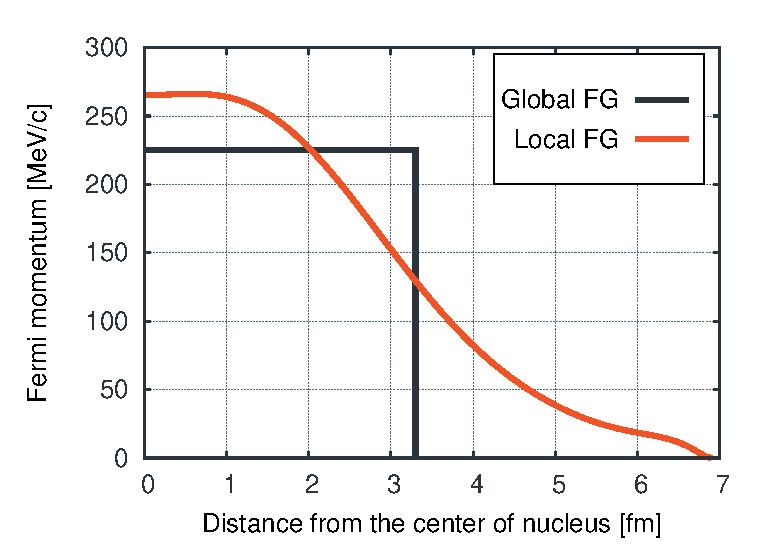
\includegraphics[width=0.5\columnwidth]{img/fermigas.eps}
  
\vfill\null
\end{slide}

%%%%% SPECTRAL FUNCTION %%%%%

\begin{wideslide}[toc=Spectral function]{Spectral function}
\null\vfill
    
  \twocolumn
  {
    \sep\sep
    \myFrame{The probability of removing of a nucleon with momentum $\vec p$ and leaving residual nucleus with excitation energy $E$.}
    $$P (\vec p, E) = P_{MF} (\vec p, E) + P_{corr} (\vec p, E)$$
    \rput[c](7.5, 2.0){\scalebox{0.75}{\begin{pspicture}
   
  \psline[linewidth = 0.025, linecolor = pdcolor6, doubleline]{<->}(-0.9,0)(-0.6,-0.75)
  
  \psline[linewidth = 0.1, linecolor = pdcolor3]{->}(-0.5,-1)(-0.2, -1.75)
  \psline[linewidth = 0.1, linecolor = pdcolor3]{->}(-1,0.25)(-1.3, 1)
   
  \pscircle[linewidth = 0.05, linecolor = pdcolor1](0,0){2}
  \pscircle[linestyle = none, fillstyle = solid, fillcolor = pdcolor1](0.75,1){0.2}
  \pscircle[linestyle = none, fillstyle = solid, fillcolor = pdcolor1](-0.5,1.25){0.2}
  \pscircle[linestyle = none, fillstyle = solid, fillcolor = pdcolor1](-1,0.25){0.2}
  \pscircle[linestyle = none, fillstyle = solid, fillcolor = pdcolor1](0,0.25){0.2}
  %\pscircle[linestyle = none, fillstyle = solid, fillcolor = pdcolor1](0.6, -0.75){0.2}
  \pscircle[linestyle = none, fillstyle = solid, fillcolor = pdcolor4](-0.5, -1){0.2}
  \pscircle[linestyle = none, fillstyle = solid, fillcolor = pdcolor1](1.25, 0){0.2}
  
  \pscoil[coilarm = 0, linewidth = 0.025, linecolor = pdcolor1, coilwidth = 0.15, coilaspect = 0]{c-c}(-2.5,0)(-1,0.25)
  \psline[linewidth = 0.025, linecolor = pdcolor1]{-c}(-3.5, -1)(-2.5,0)
  \psline[linewidth = 0.025, linecolor = pdcolor1]{-c}(-3.5, 1)(-2.5,0)
  \rput[l](-3.5,1.2){\color{pdcolor1} $l'$}
  \rput[l](-3.5,-1.2){\color{pdcolor1} $l$}
  \rput[c](0.5, -1){\color{pdcolor4} spectator}
  \rput[c]{-66}(-0.53, -0.23){\color{pdcolor6} SRC}
     
\end{pspicture}
}}
  }
  {
    \vspace*{-10pt}
    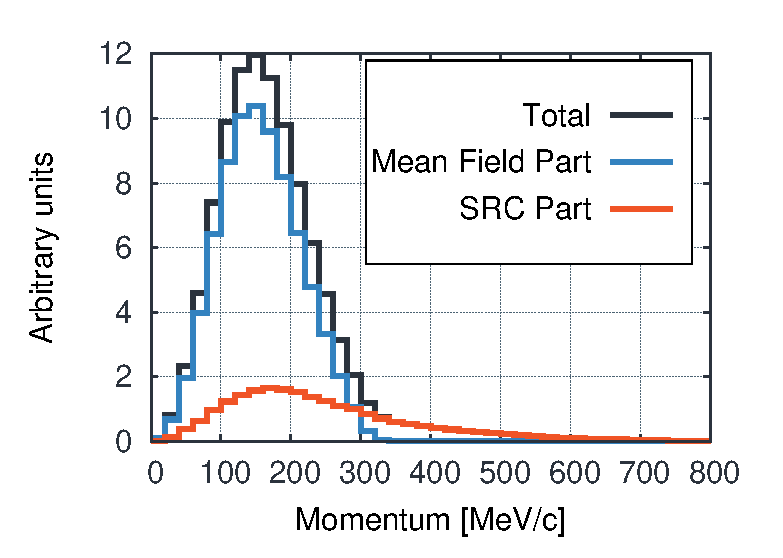
\includegraphics[width=\columnwidth]{img/sf_mom.eps}
    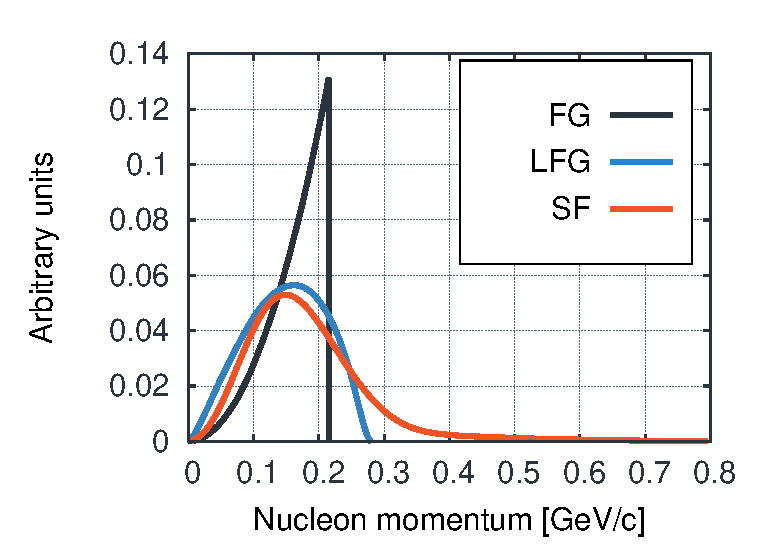
\includegraphics[width=\columnwidth]{img/fg_vs_sf.eps}  
  }

\vfill\null
\end{wideslide}

%%%%% TWO-BODY %%%%%

\begin{slide}[toc=Two-body current]{Two-body current interactions}
\null\vfill

  \sep
  \twocolumn
  {
    \begin{tikzpicture}[node distance = 0.5cm and 0.5cm]
 
  \node(tbc)  [rect, round, notFilled, minimum width = 5cm, text width = 5cm] {Two Body Current};
  \node(2p2h) [rect, round, notFilled, below=of tbc, minimum width = 5cm, text width = 5cm] {2 particles - 2 holes (2p-2h)};
  \node(mec)  [rect, round, notFilled, below=of 2p2h, minimum width = 5cm, text width = 5cm] {Meson Exchange Current (MEC)};
   
\end{tikzpicture}

  }
  {
    \rput[c](6.5, 1.6){\scalebox{0.75}{\begin{pspicture}
   
  \psline[linewidth = 0.025, linecolor = pdcolor6, linestyle=dashed]{-}(-1,0.2)(-0.55,-0.85)
  
  \psline[linewidth = 0.1, linecolor = pdcolor3]{->}(-0.5,-1)(-0.2, -1.75)
  \psline[linewidth = 0.1, linecolor = pdcolor3]{->}(-1,0.25)(-1.3, 1)
   
  \pscircle[linewidth = 0.05, linecolor = pdcolor1](0,0){2}
  \pscircle[linestyle = none, fillstyle = solid, fillcolor = pdcolor1](0.75,1){0.2}
  \pscircle[linestyle = none, fillstyle = solid, fillcolor = pdcolor1](-0.5,1.25){0.2}
  \pscircle[linestyle = none, fillstyle = solid, fillcolor = pdcolor1](-1,0.25){0.2}
  \pscircle[linestyle = none, fillstyle = solid, fillcolor = pdcolor1](0,0.25){0.2}
  %\pscircle[linestyle = none, fillstyle = solid, fillcolor = pdcolor1](0.6, -0.75){0.2}
  \pscircle[linestyle = none, fillstyle = solid, fillcolor = pdcolor1](-0.5, -1){0.2}
  \pscircle[linestyle = none, fillstyle = solid, fillcolor = pdcolor1](1.25, 0){0.2}
  
  \pscoil[coilarm = 0, linewidth = 0.025, linecolor = pdcolor1, coilwidth = 0.15, coilaspect = 0]{c-c}(-2.5,0)(-0.9,-0.35)
  \psline[linewidth = 0.025, linecolor = pdcolor1]{-c}(-3.5, -1)(-2.5,0)
  \psline[linewidth = 0.025, linecolor = pdcolor1]{-c}(-3.5, 1)(-2.5,0)
  
  \rput[l](-3.5,1.2){\color{pdcolor1} $l'$}
  \rput[l](-3.5,-1.2){\color{pdcolor1} $l$}
  \rput[c]{-66}(-0.53, -0.23){\color{pdcolor6} VM}
     
\end{pspicture}
}}
  }
  
  \vspace{-20pt}
  
  \myBoxFullWidth{Models in generators}
  
  \begin{itemize}
    \item Nieves model (GENIE, NEUT, NuWro) - CC only
    \item Transverse Enhancement model (NuWro) - both CC and NC
  \end{itemize}
  
\vfill\null
\end{slide}

\begin{wideslide}[toc=]{Two-body current interactions}
\null\vfill

  \begin{itemize}
    \item Nieves model is microscopic calculation
    \item TE model introduce $2p-2h$ contribution by modification of the vector magnetic form factors
  \end{itemize}
  
  \sep\sep

  \twocolumn
  {
    \myBox{Total MEC cross section}
    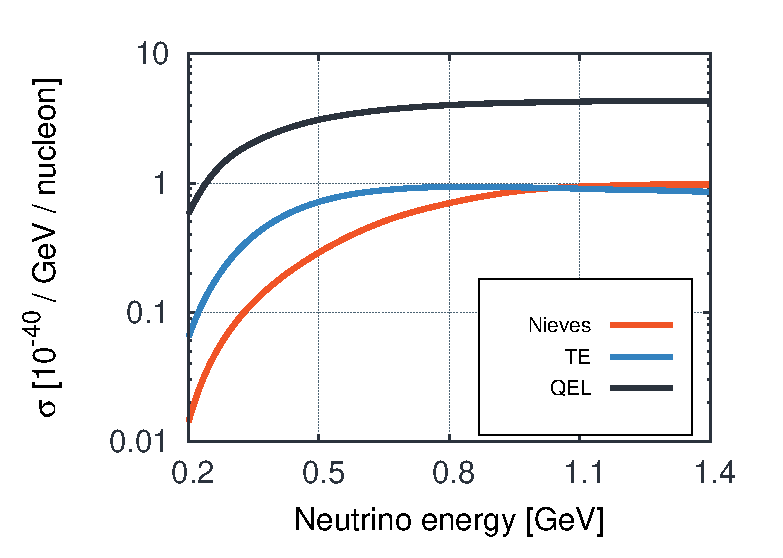
\includegraphics[width=\columnwidth]{img/mec_xsec.eps}
  }
  {
    \myBox{MEC / (QEL + MEC)}
    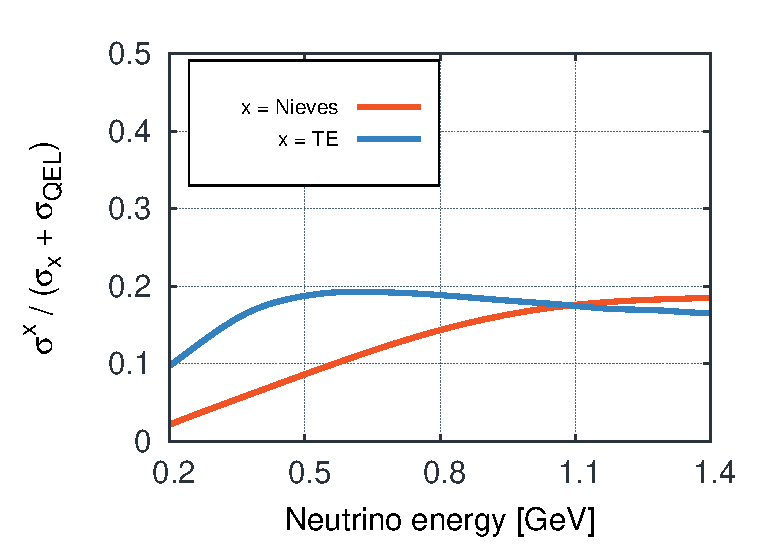
\includegraphics[width=\columnwidth]{img/mec_ratio.eps}  
  }


\vfill\null
\end{wideslide}

\begin{wideslide}[toc=]{Two-body current interactions}
\null\vfill

  \begin{itemize}
    \item Both models provide only the inclusive double differential cross section for the final state lepton
    \item Final nucleons momenta are set isotropically in CMS
  \end{itemize}

  \sep\sep
  
  \twocolumn
  {
    \myBox{Nieves}
    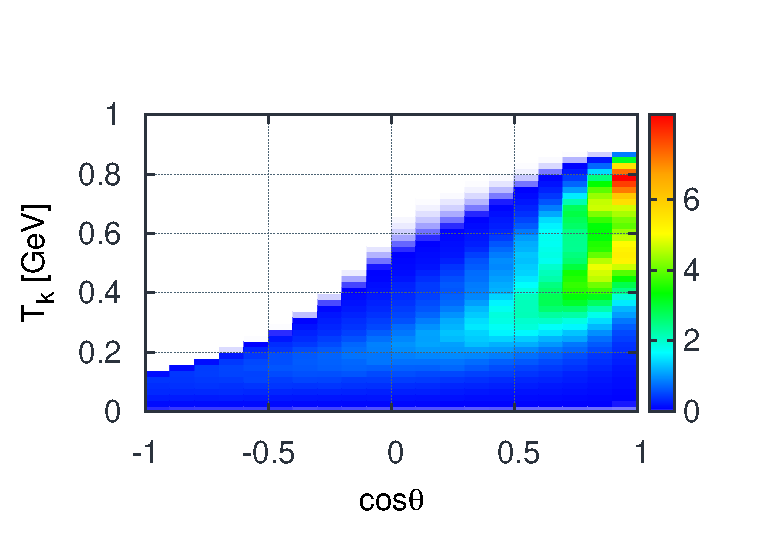
\includegraphics[width=\columnwidth]{img/mec_lep_nieves.eps}
  }
  {
    \myBox{Transverse Enhancement}
    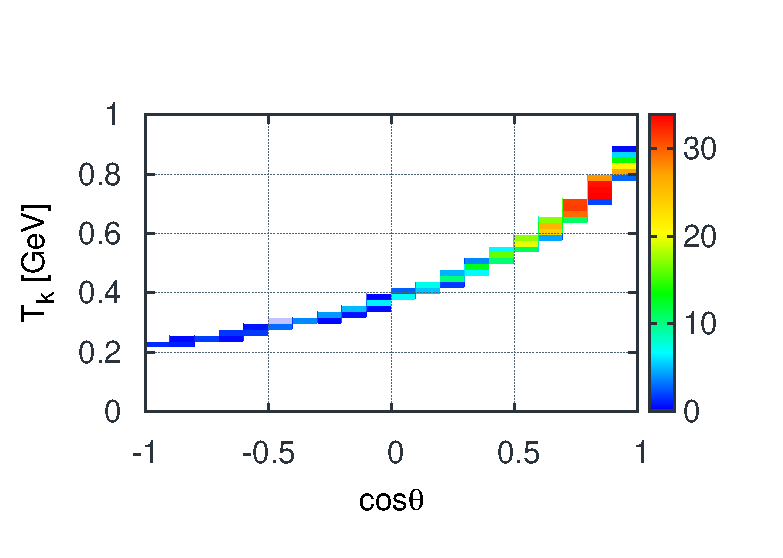
\includegraphics[width=\columnwidth]{img/mec_lep_tem.eps}
  }


\vfill\null
\end{wideslide}

%%%%% COHERENT PION PRODUCTION %%%%%

\begin{slide}[toc=COH pion production]{Coherent pion production}
\null\vfill

  \twocolumn
  {
    \begin{itemize}
      \item Rein-Sehgal model is commonly used for coherent pion production
      \item Note: it is different model than for RES
      \item Berger-Sehgal model replaces RS (NuWro, GENIE - coming soon)
    \end{itemize}
  }
  {
    \sep\sep
    \scalebox{0.75}{\begin{tikzpicture}[node distance = 1cm and 1.5cm]
  
 \node(left) [] {};
 \node(leftEmpty) [left=of left] {};
 \node(leftUp) [above=of leftEmpty] {$\nu / l$};
 \node(leftDown) [below=of leftEmpty] {$\nu$};
 
 \node(right) [right=of left] {};
 \node(rightEmpty) [right=of right] {};
 \node(rightUp) [above=of rightEmpty] {$\pi$};
 
 \node(A) [below=of right, xshift = -1cm, yshift = 0.2cm, circle, notFilled, text width = 0.75cm] {A,Z};
 \node(Aprim) [below=of right, xshift =  1cm, yshift = 0.2cm, circle, notFilled, text width = 0.75cm] {A,Z};
 
 \draw[curl, thick] (left.center) -- node[above] {$Z^0 / W^\pm$} ++ (right.center);
 
 \draw[color = pdcolor1, thick] (left.center) -- (leftUp);
 \draw[color = pdcolor1, thick] (left.center) -- (leftDown); 
 \draw[color = pdcolor1, thick] (right.center) -- (rightUp);
 \draw[color = pdcolor1, very thick, ->] (A) -- (Aprim);
 \draw[color = pdcolor1, thick, dashed, double] (right) -- ([xshift = 1cm]A.center);
 
\end{tikzpicture}
}
  }
  
  \vspace*{-10pt}
  
  \myBoxFullWidth[pdcolor3]{Comments}
  
  \begin{itemize}
    \item In COH the residual nucleus is left in the same state (not excited)
    \item The interaction occurs on a whole nucleus - no final state interactions
  \end{itemize}

\vfill\null
\end{slide}

%%%%% INTERACTIONS SUMMARY %%%%%%

\begin{slide}[toc=Summary]{Neutrino interactions - summary}
\null\vfill

  \begin{tikzpicture}[node distance = 1cm and 1cm]
 
 \node(nucleon) [notFilled={pdcolor1}, rect]                   {Nucleon (IA*)};
 \node(npnh) 	[notFilled={pdcolor1}, rect, right=of nucleon] {np-nh (semi-IA)};
 \node(nucleus) [notFilled={pdcolor1}, rect, right=of npnh]    {Nucleus};
 
 \node(neutrino) [filled={pdcolor1}, rect, round, above=of npnh] {Neutrino};
 
 \draw[line={pdcolor1}, ultra thick, ->] (neutrino.south west) -- (nucleon.north east);
 \draw[line={pdcolor1}, ultra thick, ->] (neutrino.south)      -- (npnh.north);
 \draw[line={pdcolor1}, ultra thick, ->] (neutrino.south east) -- (nucleus.north west);
 
 \begin{scope}[node distance = 0.5cm]
  \node(qel) [filled={pdcolor3}, ell, below=of nucleon] {(Q)EL};  
  \node(res) [filled={pdcolor3}, ell, below=of qel]     {RES};  
  \node(dis) [filled={pdcolor3}, ell, below=of res]     {DIS};
  \node(mec) [filled={pdcolor3}, ell, below=of npnh]    {MEC (2p2h)};
  \node(coh) [filled={pdcolor3}, ell, below=of nucleus] {Coherent $\pi$};
 \end{scope}

 \node(fsi) [filled={pdcolor4}, rect, round, minimum width = 5cm, text width = 5cm, right=of dis, xshift=0.5cm, yshift=0.75cm] {Final state interactions};
 
 \draw[line={pdcolor3}, thick, ->] (qel.south east) -- (fsi.north west);
 \draw[line={pdcolor3}, thick, ->] ([xshift=-3pt, yshift=-5pt] res.east) -- (fsi.west);
 \draw[line={pdcolor3}, thick, ->] (dis.east)       -- (fsi.south west);
 \draw[line={pdcolor3}, thick, ->] (mec.south)      -- ([xshift=-1.75cm]fsi.north);
 
 \node [below=of fsi, xshift = 2cm] {*IA = Impulse Approximation};
 
\end{tikzpicture}



\vfill\null
\end{slide}
